\documentclass[a4paper,11pt]{article}
%\documentclass[a4paper,12pt]{article}
%\usepackage[backend=biber,sorting=ydnt,maxnames=18,giveninits=true,labelnumber=true,defernumbers=true]{biblatex}
%\usepackage[backend=biber,sorting=ydnt,maxnames=18,giveninits=true]{biblatex}
%\usepackage[bibstyle=publist]{biblatex}
\usepackage{xstring}
\usepackage{url}
\usepackage{booktabs}
\usepackage{hyperref}

\usepackage{titlesec}
\titlespacing*{\section}{0pt}{12pt plus 1pt minus 0.5pt}{6pt plus 0.5pt}
%\titlespacing*{\subsection}{0pt}{5.5ex plus 1ex minus .2ex}{4.3ex plus .2ex}

\titlespacing*{\paragraph}
{0pt}{3pt plus 1pt minus 0.5pt}{3pt plus 2pt minus 0.5pt}

\usepackage{enumitem}
\setlist{nosep}

\usepackage{tcolorbox}

\usepackage{fontspec}
\setmainfont{Cambria}
\setsansfont{Calibri}

%\setlength{\itemsep}{0pt plus 1pt}
%\setlength{\itemsep}{0pt}
%\setlength{\topsep}{0pt}
\setlength{\parskip}{3pt plus 0.5pt minus 0.5pt}
%\setlength{\beforeskip}{3pt}


%\usepackage[scale=0.85]{geometry}
\usepackage[scale=0.85]{geometry}

\geometry{
 a4paper,
 total={170mm,257mm},
 left=20mm,
 top=20mm,
 }

%\assignrefcontextkeyws[labelprefix=C]{C}
%\assignrefcontextkeyws[labelprefix=J]{J}

\usepackage{fancyhdr}
\pagestyle{fancy}\lhead{Teaching Statement} \rhead{May 2019}
\chead{{\bf Dániel Varró}} \lfoot{} \rfoot{\bf \thepage} \cfoot{}

%\title{Teaching Portfolio}
%\author{D\'aniel Varr\'o}
%\date{August 2019}

\begin{document}
%\maketitle
\setcounter{page}{17}

\vspace{12pt}

%\section{Summary of Excellence}
\begin{tcolorbox}[title=Summary of Teaching Philosophy]
As a \emph{course instructor}, a main philosophy of mine is that a software engineering related course should \emph{simultaneously teach foundational concepts and cutting edge software technology}. Without the former, a course becomes empty - without the latter, a course becomes irrelevant. I am dedicated to bring \emph{realistic engineering challenges} frequently with real customers to a course that \emph{facilitate collaboration} within and between student teams while they acquire the new concepts and technologies. I regularly use various  means of \emph{active learning} to make my lectures lively. Furthermore, I always wish to maintain an \emph{inclusive atmosphere} even for a \emph{diverse and international audience}. 
\vspace{3pt}

As a \emph{supervisor} who actively collaborates with his graduate students with in-depth discussions, my goal is to continuously \emph{strive for excellence} both in engineering tasks as well as in publications while my graduate students are gradually becoming more and more \emph{independent researchers with critical thinking}.  My students typically undertake deep research tasks which go well beyond the state-of-the-art. As a further characteristic, many of our past \emph{results are simultaneously precise and scalable}, and it has been actively \emph{used in an industrial setting}. Active investment in research prototype tools help my students become \emph{excellent software engineers and architects}.
\end{tcolorbox}


%\section{Teaching Responsibilities}
%Starting as a teaching assistant in 1999, I have been involved in teaching at various levels as a full-time staff member at the Budapest University of Technology and Economics (BME, lecturing dominantly in Hungarian) between 2003 and 2016 and since then at McGill University (Canada, lecturing in English). The list of all courses I taught are listed in my CV (page \ref{xxx}).

\section{Executive summary of past teaching activities at BME}

Before joining McGill University in August 2016, I also had a long track record of teaching and course development at \emph{BME}. Below, I provide a brief executive summary only about my most significant activities at BME. 

\paragraph{Undergraduate-level teaching}
I contributed to the development and teaching of a course on \emph{Formal methods} (with 300+ students each year) since the beginning of the course in 2001 until 2006, where I also contributed three chapters in the new textbook of the course (in Hungarian).  Moreover, I was a key contributor and strategic founder of an \emph{undergraduate curriculum on Systems Engineering}.  I was major promoter and initiator of the development of an \emph{autograding software tool} (implemented by my graduate students) and subsequently used in the \emph{Systems Modeling} undergraduate course for over 5 years by now with 600+ students where each student could receive an individual technical assignment. 

In a project manager role, I participated in introducing virtual labs over educational cloud (using Apache VCL) at our faculty for the first time in Hungary which received a \href{https://inf.mit.bme.hu/en/news/2014/02/tempus-stem-call-apache-vcl-based-labs-won-prize}{TEMPUS STEM Award} in 2014. 

\paragraph{Graduate-level teaching}
At BME, I developed a course on \emph{UML-based modeling and analysis} which ran between 2003 and 2009 for 70-80 graduate (MSc) students. \emph{Several teaching assistants of the course were former students} of the course who \emph{voluntarily came back from industry to help the course}, which was a highly unusual way of teaching in Hungary. Between 2009-2016, I ran a course on “Model-driven software/systems development” (twice in English) with 15-20 students each year. I also actively contributed to start the first ever Hungarian university course on \emph{Eclipse based technologies} in 2005. I was also involved in several industrial trainings on these topics. I have been running a PhD seminar on the \emph{Foundations of Model-Driven Engineering} between 2004 and 2014 (with 5-8 students each year). 


\section{Courses Taught at McGill}
Since 2016, I taught five editions of three different courses at McGill University: ECSE 321: Introduction to Software Engineering (taught 3x), ECSE 429: Software Validation (1x), ECSE xxx: Critical Systems (1x, under temporary course code: 681) . Below, I provide an overview of the most significant course development activities are carried out in the respective courses. 
Since I only offered the ECSE 321 course more than once at McGill prior to submitting my tenure dossier, my primary focus will be on that course where the impact of my course development activities have been most apparent - and where I had chances to reflect to students' feedback I received in course evaluations.  

As the important success story for the undergraduate courses I taught (ECSE 321 and ECSE 429), I successfully integrated various cutting-edge software technologies to those courses and involved real customers/software in team projects. As a result, \emph{several students succeeded in getting summer industrial software engineering internships based solely on course material}. The graduate course, which teaches concepts and standards of model-based systems engineering, has a similar success story. Furthermore, I successfully led the development of an auto-grader software framework which can help automatically evaluate software-related assignments of students by using test cases and exploiting modern cloud-based software technologies.

\subsection{ECSE 321: Introduction to Software Engineering (Undergraduate)}
I took over this undergraduate course from Prof. Mussbacher and offered it in alternation with Prof. McIntosh who modernized many concepts taught in the course. The course covers the entire lifecycle of a modern software project including requirements engineering, domain modeling, test-driven development, continuous integration and software configuration management in the context of a group project and individual assignments. The 75-100 students of the course must have taken 1-2 previous programming courses prior to enrolling to this course. Below I highlight major developments of the course where my own initiative was predominant to improve the industrial relevance of the course, which received very positive feedback from McGill undergraduates. 
% and (2) to limit grading efforts with increasing enrollment. 

\paragraph{Modernization of software technologies and team project}
It was apparent from student feedback I received in the Winter 2017 edition of the course that the software technologies are outdated, and the students do not feel they learn modern material despite the modern concepts. Moreover, students had to develop a smaller system to three different platforms, thus they were not imposed to face integration problems which are characteristic to most modern software.

Therefore, since Winter 2018, I took the initiative and modernized the entire underlying software stack used within the course including the following specific major improvements:
\begin{enumerate}
\item The team project should \emph{develop an integrated multi-layer web application} with separate backend (i.e. services and database) and different graphical user interface frontends (mobile, web). 
\item I changed the Java-dominated technological stack to include \emph{heterogeneous technologies} including a modern web technologies (like HTML5, JavaScript or Vue.js), a modern backend technology (JavaSpring, RESTful API), and Gradle for build automation. I also included respective programming concepts such as asynchronous method calls or promises. 
\item I introduced a proper underlying relational database technology on top of an object persistence layer using the standard Java Persistence API. I developed respective lecture material to cover the basic concepts of relational databases (as students take the Database course later) and the standard \emph{object-relational mapping}.  
\item While Montreal is a major aerospace hub, the existing courses of the software engineering curriculum failed to offer specific insights in engineering critical systems. Therefore, I developed lectures on \emph{platform-based design in systems architecture} as well as the \emph{foundations of fault-tolerant systems}.
\end{enumerate}

Since the theme of the software engineering team project was different in every year, students could decide if they wish to open their GitHub repositories that stored the source code of their projects after the completion of the course. Many teams opted for an open repository and \emph{students started to use their ECSE 321 project as a reference work during interviews of summer internship}. This is clear indication of the industrial usefulness and practical effectiveness of the course as a result of the changes above. 

\paragraph{Involving real customers in team projects}

To better motivate students, I put extra emphasis on providing real challenges for the complex software engineering project carried out by teams. Therefore, I selected project themes where McGill employees could serve as real customers. Those customers participated in requirements engineering sessions where students could ask questions to clarify the scope of the project. Moreover, these customers also attended (and graded) the final student presentations and the final software artifact.
\begin{itemize}
\item In Winter 2018, student teams had to develop a software application to manage and supervise the trees in Montreal and calculate various forecasts for evaluating sustainability attributes. Many details of the project were proposed by Prof. Andrew Gonzalez, Prof. Kevin Manaugh and Prof. David Wachsmuth who offered their continuous involvement.
\item In Winter 2019, student teams had to develop an application to help manage co-op programs (i.e. curricula with compulsory industrial internship) at McGill University. In this case, Ms. Lorraine Donald (Industrial Liason Associate and future administrative coordinator of the upcoming software engineering co-op program) offered continuous help during the project. Moreover, final presentations of student teams were also attended by various employees at the Faculty of Engineering.
\end{itemize}


\paragraph{Redevelopment of tutorials: contents and technology}
As a consequence of the above initiative, the \emph{sample project as well as the technical contents of the tutorials of the course had to be redeveloped from scratch} which I carried out together with Márton Búr, my PhD student (with further initial help from my graduate students at BME, Gábor Szárnyas and Oszkár Semeráth). This was a major investment since the total length of the PDF version of the material was 75-100 pages. 

To improve the maintainability of tutorial materials, I promoted to host those tutorial materials on GitHub and continuously compile changes into a new version of the document available both in HTML and PDF formats (see e.g. 
\href{https://mcgill-ecse321-winter2019.github.io/EventRegistration-Tutorials/}{ECSE321-W2019}, 
\href{https://mcgill-ecse321-winter2018.github.io/EventRegistration-Tutorials/}{ECSE321-W2018}, 
\href{https://ecse321-winter2017-mcgill.github.io/EventRegistration-Tutorials/}{ECSE321-W2017}). As such, even the tutorials of the course actually used the same software technologies (Gradle, Github, TravisCI) taught by the course. 



\paragraph{Auto-grader for individual software technology assignment}
To assure that all students taking the course successfully learned not only the core concepts but also the key software technologies, a programming assignment has already been an integral part of the course where students had to develop a small-scale web application using the same technologies as in the large-scale group project. This assignment had to be carried out by the students either in pairs (in 2017 and 2018) or individually (in 2019). 

However, the evaluation of these individual assignments has been very laborious and somewhat subjective and error-prone. Therefore, I took the initiative to develop an auto-grader framework that could automatically evaluate student submissions by running predefined test cases. The key concepts of the auto-grader framework are the following:

\begin{itemize}
\item Each student needs to develop a unique combination of software features by extending a baseline web application made available to them as a starting point. All development needs to be done in an individual (private) GitHub repository of the student (identified by their McGill IDs). The individual specification of the assignment is also generated automatically for each student. 
\item The auto-grader evaluates student submission by running a dedicated test suite. The Instructors need to develop the superset of all test cases from which the auto-grader selects the ones required for the features addressed by the specific student. 
\item The 80\% of the test cases are made publicly available to students so that they can use them as a reference while developing their solution. The remaining 20\% of the test cases were only included in the official grading process. 
\item The actual grading is carried out as part of a continuous integration process, which automatically builds the student project, then executes the relevant set of test cases, and finally reports the evaluation in a separate GitHub branch.
\end{itemize}

The auto-grader has been successfully used in Winter 2019, but several colleagues at my department has expressed there interest in potetially adapting the framework to their course. 

\paragraph{Undergraduate students as project mentors}
With the help of the Tomlinson Engagement Award for Mentoring (TEAM), I systematically involved excellent undergraduate students in the next edition of the ECSE 321 course. A total of six TEAM mentors (in 2018 and 2019) successfully helped team projects to overcome the difficulties of integrating various software technologies. Moreover, they also helped develop the auto-grader framework. While the TEAM award is on a nomination basis, several undergraduates have indicated to volunteer for the next year, which clearly demonstrates the positive impact of this change.


\subsection{ECSE 429: Software Validation (Undergraduate)}

I gave this undergraduate course in Fall 2018 for over 120 students - most of who were taking this course just before their graduation. The course covers various techniques of software quality assurance including testing, static analysis and formal verification. The students of the course need to complete a complex software testing project (in teams) as well as individual testing assignments and three quizzes.

Since the lecture material of the course has been recently redeveloped (by Prof. Mussbacher), I built upon and reused significant amount of existing course material. Since the software technologies used within the course were outdated, my primary goal was to increase the practical and industrial impact of the course by the following initiatives:

\begin{enumerate}
\item The \emph{tutorials of the course have been redesigned almost from scratch} (with contributions from the two teaching assistants, Márton Búr and Mathieu Boucher). New material included the introduction of code reviews, continuous integration, modern static analysis tools (SonarQube, Infer), automated test case generators (EvoSuite), various frameworks for integration testing as well as end-to-end testing Android applications, model-based testing tools. I adapted the use of GitHub for hosting the \href{https://mcgill-ecse429-fall2018.github.io/Tutorial-Lecture-Notes/}{material of the tutorials}, which allows that corrections can be immediately published to the live material (without extra manual document upload). 

\item As being of utmost importance in modern software quality assurance, I \emph{developed course material related to code reviews and and static analysis techniques} as part of the lectures and introduced an extra deliverable for the team project. To further increase practical relevance, the introductory materials of software quality assurance and testing has been aligned with contents and recommendations of the International Software Testing Qualifications Board (ISTQB) for foundation level certification.

\item Within the complex team project of the course, \emph{student teams had to test a real open source Android application} (Blokish game). Although the suitability of this very project was criticized by students, they were simultaneously enforced to understand and handle the imperfections of real software projects, which is frequently the case in real software projects. 

\item To avoid the laborious work of grading the three individual quizzes with an increased number of enrolled students, I \emph{changed the former closed-book in-class quizzes into an open-book, online quizzes} evaluated semi-automatically using existing support in MyCourses. Students had to complete each quiz in 75 minutes within a 6-hour time-frame, which gave them extra flexibility to avoid clashes of midterm exams with other courses, and in general, it reduced the perceived stress level. 
\end{enumerate}

\subsection{ECSE xxx/681: Critical Systems (Graduate)}

I proposed and \emph{developed a brand new graduate course on Critical Systems} to provide an overview of main challenges and activities in the design and assurance of critical software-intensive cyber-physical systems (CPSs). The first part of the course is dedicated to the core concepts, languages and techniques of model-based systems engineering used for designing such systems while covering key concepts like safety cases, traceability, viewpoints of system architecture, design space exploration, etc. In this first part, students carry out a complex design project using standard modeling languages (like SysML, Capella) and simulation tools in the context of a cyber-physical system or Internet-of-Things application. This first part is complemented with in-class tutorials and modeling workshops to help students effectively use complex industrial systems engineering tools.

The second part of the course is dedicated to assurance critical CPSs to guarantee the safe behavior of such systems by discussing a wide range of design-time and run-time assurance techniques. In the second part, students familiarize themselves with research results used for the assurance of such systems including various approaches of verification and validation (V\&V). The end of the course is dedicated to recent research challenges for the safety assurance of autonomous systems driven by machine learning and other AI techniques. These research-related contents are close to my own research area, thus student presentations of various research topics normally involve lively and deep discussions. 

I offered the first edition of the course (under a temporary course code) in Winter 2018 for 18 graduate students. As an extra research component for this first edition, students had to assemble a survey presentation of a research topic by categorizing over 15 papers. The official approval of the course is ongoing, and it is expected to be completed in Fall 2019. 


%\paragraph{Undergraduate-level courses.}

%At \emph{McGill University}, I was the instructor of a course on \emph{Introduction to Software Engineering} for three times with 75-95 students in 2017-2019 and for a very diverse and international audience. In all three editions, I received an average score between 4.2-4.5 (out of 5.0) for all course evaluation questions related to me as instructor, which was significantly over the department average (by an average of 0.6). In 2018, I significantly modernized the technological background of the course – which now teaches modern software engineering principles and architectures in the context of modern software technologies. Despite the heavy workload, the vast majority of students loved the course and gave very positive feedback, such as “\emph{It has been the most interesting and educational course I have taken. So much effort is put in this course from the detailed \href{https://mcgill-ecse321-winter2019.github.io/EventRegistration-Tutorials/}{Hands-On tutorial} document, to the project requirements supported by ‘real’ clients, and finally, the \href{https://flipquiz.com/flashcards/82085/}{interesting games}!}”, “\emph{Professor Varro is by far one of the most helpful, dedicated professors at McGill}”. At McGill, I voluntarily took several trainings offered by Teaching and Learning Services at McGill on how to increase student participation by \emph{active learning} (e.g. frequent online polls during lectures). In Fall 2018, I also taught a course on \emph{Software validation} for over 120 students, but future editions of this course will need significant further modernization.

%\paragraph{Graduate-level courses.}
%At McGill University, I offer a graduate course on 
%\emph{model-based engineering for cyber-physical systems} 
%\emph{critical systems} ()
%which teaches SysML and related standards in the context of Internet-of-Things and safety-critical CPS.

\subsection{Evidence of Teaching Effectiveness at McGill}

\subsubsection{Course Evaluation Results}

\autoref{tab:course-eval} shows the course evaluation results for all the 14 regular questions for the five course offerings I have taught at McGill since Fall 2016. The four main questions (Q1 to Q4) are highlighted in bold, whereas additional instructor-specific questions (Q3-Q8) are printed in italics. The department means (DM) are shown in parentheses in the table to enable certain comparison. 

\begin{table}[htbp]
\footnotesize
\begin{tabular}{@{}p{8cm}p{1.3cm}p{1.3cm}p{1.3cm}p{1.3cm}p{1.3cm}@{}}
\toprule
\textbf{Question} & \textbf{ECSE321} \newline \textbf{W17} \newline \textbf{(DM)} & 
\textbf{ECSE321} \newline \textbf{W18} \newline \textbf{(DM)} & 
\textbf{ECSE321} \newline \textbf{W19} \newline \textbf{(DM)} & 
\textbf{ECSE429} \newline \textbf{F18} \newline \textbf{(DM)} & 
\textbf{ECSE681} \newline \textbf{W18} \newline \textbf{(DM)} \\ \toprule
Response rate (\%) & 44 & 47 & 44 & 34 & 67 \\ \midrule
\textbf{Q1: Overall, this is an excellent course.} & \textbf{3.8} \newline (3.8) & \textbf{4.5} \newline (3.8) & \textbf{4.4} \newline (3.8) & \textbf{3.6} \newline (3.8) & \textbf{3.9} \newline (3.8)  \\ \midrule

\textbf{Q2: Overall, I learned a great deal from this course.} & \textbf{4.2} \newline (4.0) & \textbf{4.5} \newline (3.9) & \textbf{4.4} \newline (4.0) & \textbf{3.9} \newline (4.0) & \textbf{3.7} \newline (3.9)  \\ \midrule

\textbf{Q3: Overall, this instructor is an excellent teacher.} & \textbf{4.3} \newline (3.7) & \textbf{4.4} \newline (3.7)  & 
\textbf{4.5} \newline (3.8)  & \textbf{4.0} \newline (3.9) & \textbf{4.6} \newline (3.7)  \\ \midrule

\textbf{Q4: Overall, I learned a great deal from this instructor.} & \textbf{4.2} \newline (3.7) & \textbf{4.3} \newline (3.7)  & 
\textbf{4.3} \newline (3.8) & \textbf{4.0} \newline (3.9) & \textbf{4.3} \newline (3.7) \\ \midrule

\emph{Q5. The instructor was well organised in class and presented the material clearly.} & 4.1 \newline (3.7)  & 4.2 \newline (3.7)  & 4.4 \newline (3.9)  & 4.0 \newline (4.0) & 3.5 \newline (3.7) \\ \midrule

\emph{Q6. The instructor used effective teaching methods.} & 4.2 \newline (3.6)  & 4.2 \newline (3.7) & 
4.2 \newline (3.7)  & 3.7 \newline (3.7)  & 3.8 \newline (3.6) \\ \midrule

\emph{Q7. The instructor was responsive to students’ questions and concerns, given the class size.} & 4.5 \newline (4.2)  & 4.7 \newline (4.1) & 4.5 \newline (4.2)  & 4.3 \newline (4.2) & 4.9 \newline (4.1)  \\ \midrule

\emph{Q8. The instructor fostered an environment of mutual respect and engagement in learning.} & 4.7 \newline (4.2)  & 4.8 \newline (4.1) & 4.7 \newline (4.1)  & 4.3 \newline (4.2) & 5.0 \newline (4.1)  \\ \midrule

Q9. The course materials contributed to learning the subject matter. & 4.2 \newline (4.0)  & 4.5 \newline (4.0) & 
4.2 \newline (4.0)   & 4.0 \newline (4.1) & 3.3 \newline (4.0)  \\ \midrule

Q10. The course activities (inside and outside the classroom) engaged me actively in my learning process. & 4.4 \newline (3.8)  & 4.6 \newline (3.8) & 4.3 \newline (3.8)  & 3.8 \newline (3.9) & 4.2 \newline (3.8)  \\ \midrule

Q11. The evaluation methods used in this course were fair and appropriate. & 4.2 \newline (3.7)  & 4.3 \newline (3.8) & 
4.2 \newline (3.8)  & 3.8 \newline (3.8)  & 4.2 \newline (3.8) \\ \midrule

Q12. I was provided with useful feedback on my progress in the course. & 3.8 \newline (3.7)  & 4.4 \newline (3.6)  & 
4.4 \newline (3.8)  & 3.5 \newline (3.7)  & 4.1 \newline (3.6) \\ \midrule

Q13. The course workload was appropriate, given the credit weight and the scheduled activity hours. & 3.5 \newline (3.7)  & 3.5 \newline (3.8)  & 3.5 \newline (3.8)  & 3.3 \newline (3.7)  & 4.2 \newline (3.7) \\ \midrule

Q14. As a result of this course, I have a greater appreciation for the relevance of this topic to my chosen profession. & 4.3 \newline (3.9)  & 4.4 \newline (3.8)  & 4.4 \newline (3.8)  & 3.6 \newline (3.9)  & 3.9 \newline (3.9)  \\ \midrule

\bottomrule
\end{tabular}
\caption{Course evaluations}
\label{tab:course-eval}
\end{table}

\paragraph{General feedback}

The course evaluations of all courses I taught at McGill are consistently very high. Over 82\% of the results (58 out of 70 cases) exceed the department mean (DM), while in 44\% of the cases (31 out of 70 cases), the results are significantly higher than the DM (by at least 0.5 points). There is a single question (Q13) about the appropriateness of the course workload where my scores are repeatedly below the DM. However, all of my courses are project-based, which, in general, requires more work from students. Moreover, certain efforts invested by students in those courses are actually voluntary work (i.e. students aimed for bonuses). As such, students normally work a lot in my courses, but they also learn a lot from them. 

The results for the four core questions (Q1-Q4) are over 4.0 in 75\% of the cases (15 out of 20). Morever, all of the results were over 4.3 for repeated editions of the same course (ECSE 321), which shows that I succeeded in making necessary adaptations to subsequent editions of the course once I grasp the general background knowledge of students. 

My instructor-specific evaluations (Q3-Q8) are excellent: almost all cases (93.3\%, 28 out of 30) exceed the DM; while, 63.3\% (19 out of 30 cases) exceeds the DM by a large margin (over 0.5 points).  In general, students seem to be very supportive of my teaching style as shown by the fact that 90\% (27 out of 30) of my instructor scores are over 4.0.




%When teaching the course for the first time in Fall 2018, I decided to significantly upgrade and modernize the underlying software quality assurance technologies and tutorials used in the course, and changed the scope of the complex team project to test Android applications, while I reused significant amount of existing course material, thus interpreting the results needs some extra caution. 




\subsubsection{Technological self-evaluation of students}
In addition to Mercury course evaluations, since Winter 2018, I have voluntarily collected self-evaluations of students in the form of online polls. The same questionnaire was voluntarily filled by students twice: once during the first lecture and once during the final lecture. My goal is two-fold (1) to assess the entry level of students related to key technologies covered in a course and (2) to obtain a technical feedback about the technological progress of students during the course. 

The measurement of technological progress of students in software engineering courses is of utmost importance from a practice-oriented perspective: the vast majority of technical descriptions in software engineering jobs refer to technologies rather than concepts. As such, students must simultaneously acquire concepts and technologies as part of their undergraduate training in a rapidly changing technological environment. 

The results of the technological self-evaluation of students for the two undergraduate courses are presented in \autoref{tab:tech-eval-ecse321} and \autoref{tab:tech-eval-ecse429}.



\begin{table}[htb]
\footnotesize
\begin{tabular}{@{}p{8cm}p{1cm}p{1cm}p{1cm}p{1cm}p{1cm}p{1cm}@{}}
\toprule
\textbf{ECSE 321 Questions} & 
\textbf{W18} \newline \textbf{Begin} & 
\textbf{W18} \newline \textbf{End} & 
\textbf{W18} \newline \textbf{Incr} & 
\textbf{W19} \newline \textbf{Begin} & 
\textbf{W19} \newline \textbf{End} &
\textbf{W19} \newline \textbf{Incr} \\ \toprule
Participants (\#) & 64 & 43 &  & 80 & 32 &  \\ \midrule
I am familiar with Java as a programming language. & 1.54 & 1.36 & \textbf{0.18} & 1.45 & 1.24 & \textbf{0.21} \\ \midrule

I am familiar with JavaScript as a programming language. & 3.75 & 2.66 & \textbf{1.09} & 3.90 & 2.61 & \textbf{1.29} \\ \midrule

I am familiar with Java Spring or RESTful services. & 4.60 & 2.05 & \textbf{2.55} & 4.68 & 1.83 & \textbf{2.85}  \\ \midrule

I am familiar with Android applications. & 4.39 & 2.54 & \textbf{1.85} & 4.52 & 4.19 & \textbf{0.33}   \\ \midrule

I am familiar with a modern web frontend technology (e.g. Vue.js, React, Angular or similar). & 4.61 & 2.92 & \textbf{1.69} & 4.36 & 2.23 & \textbf{2.13}  \\ \midrule

I am familiar with database technologies (e.g. Hibernate, MySQL or similar). & N/A & N/A & & 
4.18 & 2.41 & \textbf{1.77}  \\ \midrule

I am familiar with UML (the standard modeling language). & 3.80 & 1.75 & \textbf{2.05} & 
2.90 & 1.76 & \textbf{1.14}  \\ \midrule

I am familiar with coding conventions (or other techniques for developing clean source code). & 2.32 & 1.71 & \textbf{0.61} & 2.35 & 1.93 & \textbf{0.42}   \\ \midrule

I am familiar with testing principles or technologies.
& 3.53 & 1.78 & \textbf{1.75} & 3.89 & 2.03 & \textbf{1.86}  \\ \midrule

I am familiar with Git as a version control system.
& 2.51 & 1.29 & \textbf{1.22} & 2.23 & 1.20 & \textbf{2.13}  \\ \midrule

I am familiar with modern automated build or continuous integration technologies (e.g. Gradle, Maven, Travis, Jenkins).
& 4.48 & 2.61 & \textbf{1.87} & 4.29 & 2.13 & \textbf{2.16}  \\ \midrule

\bottomrule
\end{tabular}
\caption{Averages of students' technological self-evaluation in ECSE 321 course at the beginning and at the end of course on a Likert scale (1: strongly agree, 2: somewhat agree, 3: neutral, 4: somewhat disagree, 5: strongly disagree ) }
\label{tab:tech-eval-ecse321}
\end{table}

\begin{table}[htb]
\footnotesize
\begin{tabular}{@{}p{12cm}p{1cm}p{1cm}p{1cm}@{}}
\toprule
\textbf{ECSE 429 Questions} & 
\textbf{F18} \newline \textbf{Begin} & 
\textbf{F18} \newline \textbf{End} & 
\textbf{F18} \newline \textbf{Incr} \\ \toprule
Participants (\#) & 85 & 39  \\ \midrule
How familiar are you with JUnit (or other unit testing technology)? & 1.97 & 1.86 & \textbf{0.11} \\ \midrule

How familiar are you with mocking technologies like Mockito (or similar)? & 3.46 & 2.06 & \textbf{1.40} \\ \midrule

How familiar are you with advanced static analysis tools like SonarQube or Infer? & 3.68 & 2.14 & \textbf{1.54} \\ \midrule

How familiar are you with advanced code review tools like Gerrit or ReviewBoard? & 2.76 & 2.22 & \textbf{0.54} \\ \midrule

How familiar are you end-to-end brower testing technologies? & 3.28 & 2.97 & \textbf{0.31}  \\ \midrule

How familiar are you with story testing or behavior driven development technologies like Cucumber? &
3.53 & 2.64 & \textbf{0.89}  \\ \midrule

%How familiar are you with model-based testing technologies like GraphWalker? & 3.92 & 3.46 & \textbf{0.46} \\ \midrule

How familiar are you with code-based test generation technologies (like EvoSuite)?
& 3.92 & 2.28 & \textbf{1.64} \\ \midrule
\bottomrule
\end{tabular}

\caption{Averages of students' technological self-evaluation in ECSE 429 course at the beginning and at the end of course on a 1-to-4 Likert scale (1: I used it in industrial project during my work or an internship, 2: I used it in a software engineering project in one or more courses, 3: I learned about it in a tutorial, but have not used it on my own, 4:
I do not know about it)}
\label{tab:tech-eval-ecse429}
\end{table}

\paragraph{Evaluation of students' technological progress}

Altogether, the students have made a remarkable technological progress related to the majority of technologies in both courses, which is a substantial pedagogical achievement for all instructors and teaching assistants involved in the course. This success can be attributed to (1) the extensively redeveloped tutorials and (2) the fact that they had to apply technologies in a complex software engineering team project (which naturally caused an increased student workload).  As such, it truly reflects the effectiveness of my course development activities. 

\begin{itemize}
\item \textbf{ECSE 321:} In both editions, at the beginning of the semester, students were only familiar with Java and somwhat familiar with coding conventions and UML. By the end of the semester the technological level of students was lower than 3.0 for all technologies (except for Android in Winter 2019 which was turned into an optional project deliverable due to scheduling constraints) and below 2.0 for 5 out of 10 technologies (i.e. better than at least somewhat familiarity). Students had an improvement over 1.0 (out of a 5 point Likert scale) for 8 out of 10/11 technologies. It is very important to emphasize that students were totally unfamiliar with 5 out of 10 technologies in the beginning (with a score over 4.0), and they could simultaneously make technological progress in most of the technologies. 

\item \textbf{ECSE 429:} Again, major technological improvement has been made by students in most of the key technologies covered in the tutorials of the course, especially, in the case, when students had to use a given technology in the context of a complex software quality assurance project. Technological progress exceeded 0.5 (on a 1 to 4 scale) for 5 out of 7 technologies, and students only had difficulties in acquiring end-to-end browser testing technologies.
\end{itemize}

\subsubsection{Further teaching practices for students' positive learning experience}

There are several techniques I repeatedly apply in my lectures to facilitate a positive learning experience for students and make the classroom more inclusive. I provide a brief summary of the key techniques that I successfully used in multiple courses. 

\paragraph{Questions by online polling}
In general, I limit the presentation of new material to 15 minutes at most, which is followed by some other activities. As part of that, I regularly ask questions during my lectures to keep the students involved, I realized that this is not very effective with for students who are rather shy or introverted. Therefore, I regularly ask questions in the form of online polls where all students with a laptop or a mobile phone can participate and share their views or test the correctness of their answers. 

\paragraph{Technological exercises}
While technologies are traditionally covered only at tutorials and lectures are primarily focusing on teaching novel concepts, concepts and technologies are not always separable in case of modern software. Therefore, I regularly include short 5-10 minute technological exercises during my lectures what needs to be completed by students on their own laptops. For example, teaching state-of-the-art version control systems (such as Git) or automated builds (like Gradle) is more effective that way in my view. 

\paragraph{Games as midterm/final exam review}
I find it very important to regularly review the material covered in the class even (if there are no related quizzes or midterm exams). To make such occasions more interactive, I regularly use games where teams can compete against each other or they need to collaboratively solve particular tasks. A sample screenshot from the Jeopardy game I repeatedly used in the ECSE 321 course is given in \autoref{fig:jeopardy-ecse321}. After the game, all questions are made available online for the students as additional review preparation material.

\begin{figure}[htb]
\centering
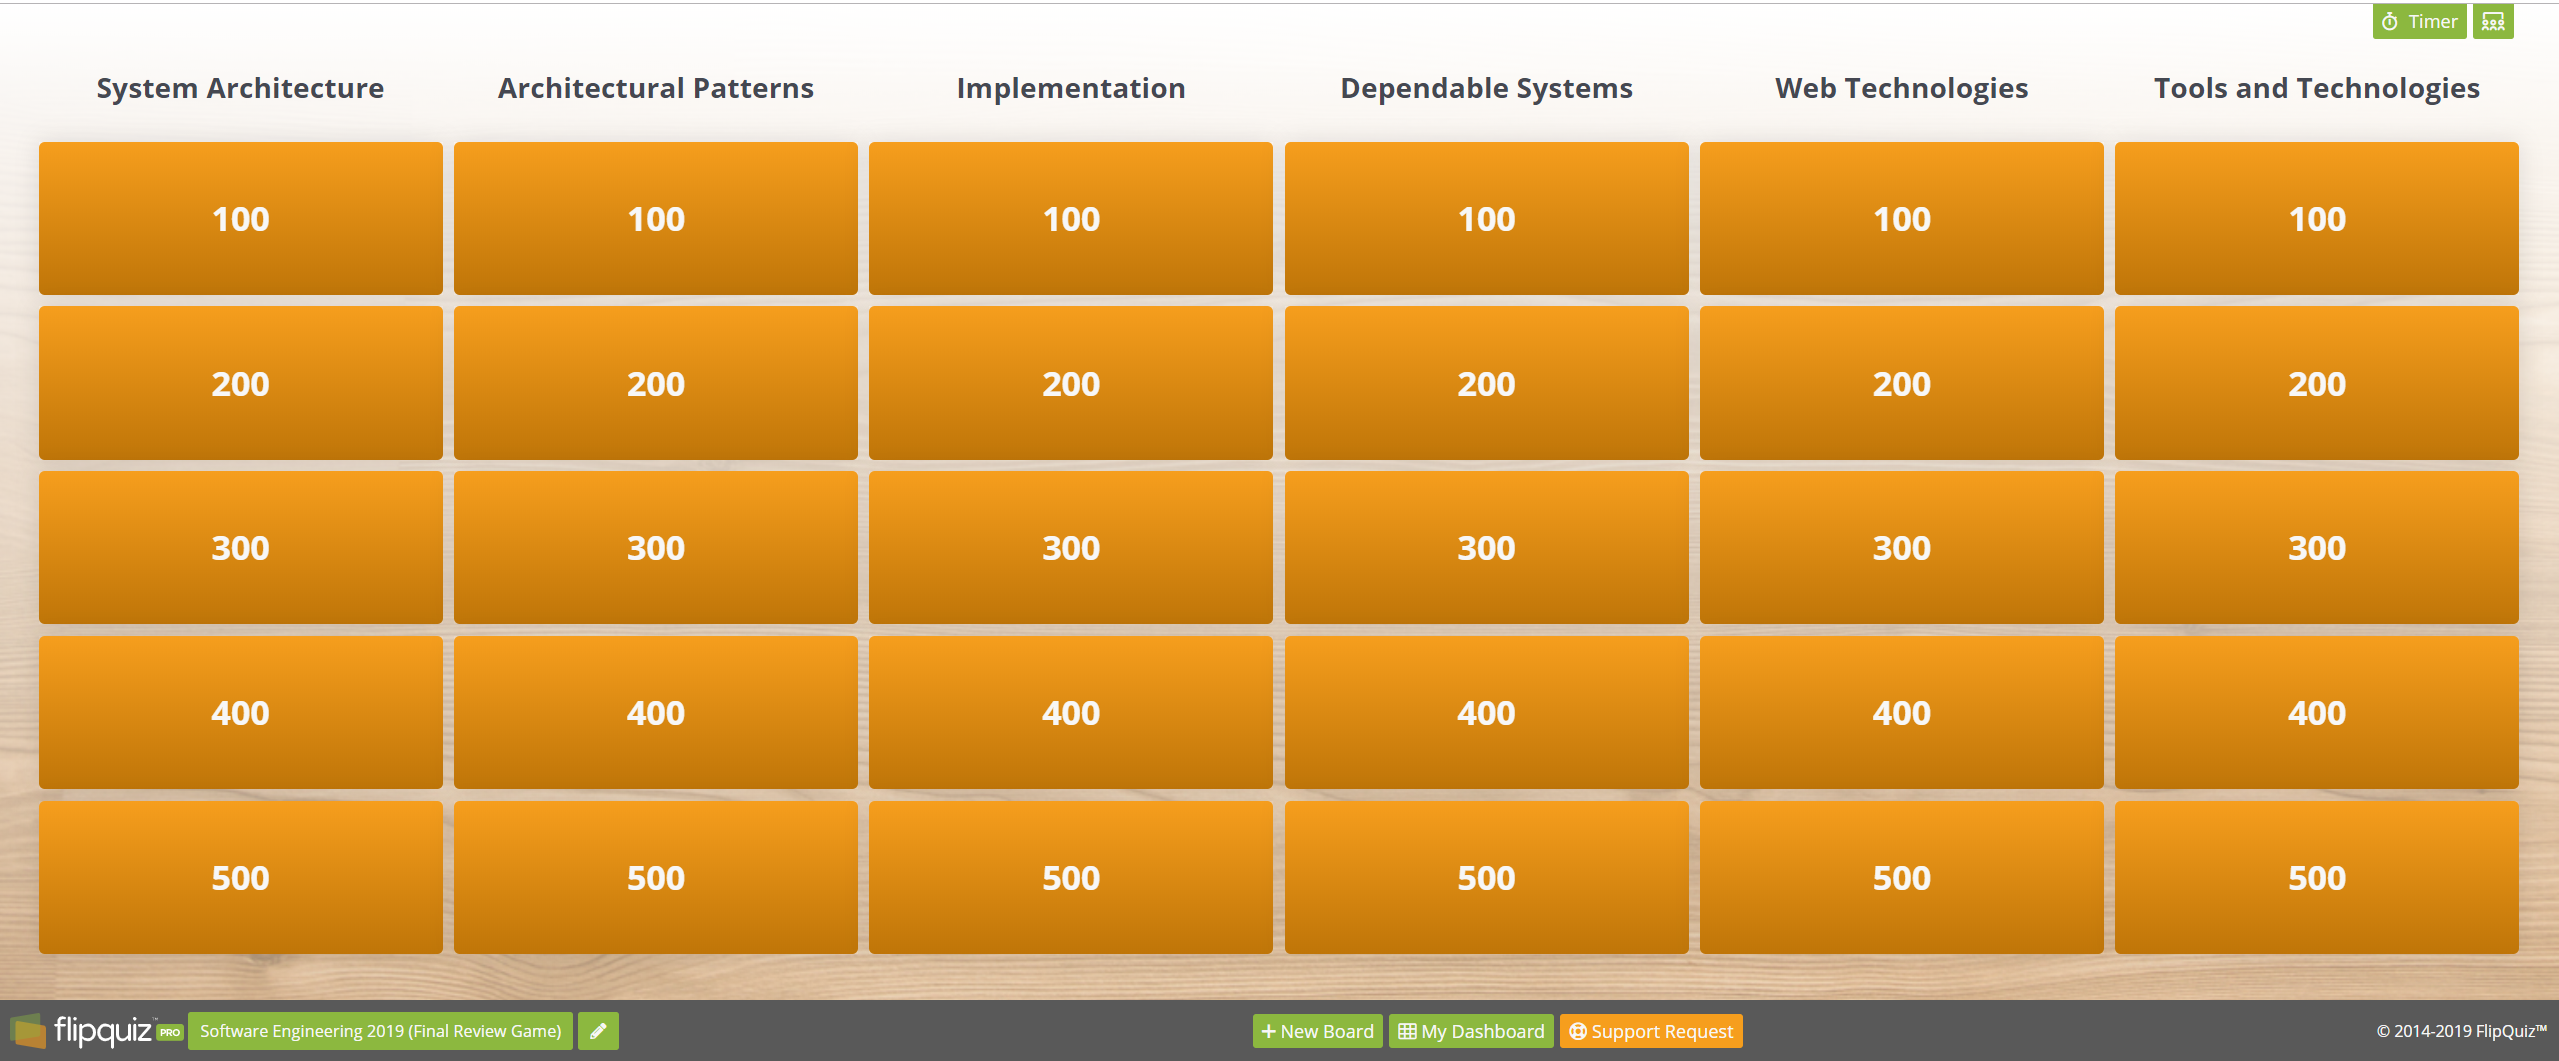
\includegraphics[width=.8\textwidth]{figures/FlipQuiz}
\caption{Jeopardy game in ECSE 321: Introduction to Software Engineering course}
\label{fig:jeopardy-ecse321}
\end{figure}



\paragraph{Course-specific feedback: ECSE 321}
Based on the textual feedback I received in Winter 2017, I decided to modernize the underlying software technologies used in the complex team project. As result, all scores for all questions in the Winter 2018 and Winter 2019 editions of the course reached at least 4.2 - and improved with respect to the Winter 2017 edition in all but one cases. 

A complete set of textual comments received from students of the ECSE 321 course is reproduced in Appendix~\ref{xxx}. A few representative excerpts are given below:
\begin{itemize}
\item TODO
\end{itemize}

Altogether, I was a key initiator to evolve a very good course into an excellent one, which is frequently regarded by undergraduate students as the flagship course of the software engineering curriculum which helps student find internships at high-tech software companies. After introducing new software technologies, modernizing the tutorials and bringing real customers of the team project, the complex team software projects serve as a first reference work for many students. 

\paragraph{Course-specific feedback: ECSE 429}
The course evaluations of ECSE 429 are lower than that of ECSE 321, but the results are generally close to the department mean, so they are fine when teaching a course for the first time. There are three negative outliers, namely, Q12, Q13 and Q14 which need further action in the future. 

\begin{itemize}
\item Q13: The very high workload was dominantly caused by (1) selecting a real open source Android project as the subject of the team software quality project, which turned out to be too real as students complained about the low quality of the source code. Moreover, (2) students had to complete three assignments and three on-line quizzes during the semester. Since a real quality assurance project is very important part of the course in my view, in the future, I plan to turn the three extra assignments to be bonus exercises. As such, the exercises are still there for preparing of the final exam, but the amount of compulsory work is reduced. 

\item Q12: The lack of timely feedback was caused by the increased workload of graders. By removing the three compulsory assignments, the workload of the graders will also be reduced. 

\item Q14: Many students take the ECSE 429 course during their final semester at McGill, and as such, frequently after an industrial internship/work experience. Therefore, they might already be familiar with a significant part of the course content. Unfortunately, it is impossible to force these students to take this course earlier due to scheduling constraints. 

\end{itemize}


\paragraph{Course-specific feedback: ECSE 6xx: Critical systems}
While I have over 15 years of experience in teaching various masters-level graduate courses in Hungary, I had some very unexpected experience during the first edition of the ECSE 6xx course on Critical Systems I gave at McGill University as a result of a mutual mismatch of expectations. The majority of graduate students who took my course required were not really independent thinkers and they required much more hand-holding than I ever gave during a graduate course. As I used some of the teaching material in the past for industrial trainings on the standard SysML modeling language, the lower score (3.3) on course material is especially surprising.

Based on the experience and feedback, there are two ways to proceed: either (1) the course should be more research-intensive (when the course enrollment may be significantly lower), or (2) it should be turned into lower-level course with both graduate and (higher-year) undergraduate students (with higher enrollment, but less research content). 


%\subsubsection{Final reflections}

%\paragraph{Course-specific reflections: ECSE 321}

%\paragraph{Course-specific reflections: ECSE 429}



\section{Talent Care and Student Supervision}
\paragraph{Supervising PhD and MSc theses.}
Starting from my early PhD studies, I have been active in talent care by supervising MSc and PhD students. I have been the \emph{main scientific advisor of 11 PhD students} (5 completed, 3 PhD candidates to complete in Summer 2019), and co-supervised 3 more PhD students (2 completed, 1 PhD candidate). I also supervised 20+ MSc theses since 2001. All of my \emph{seven best paper awards had one of my PhD students} as the first author. Moreover, my PhD students were successfully competing at prestigious international Student Research Contests and Doctoral Symposiums (2x 1st prize at MODELS, 1x 2nd prize at SIGMOD, 1x 1st prize at STAF conferences).

\paragraph{Supervising early research work.} 
23 scientific reports written by MSc students under my tutoring participated successfully in a national two-phase (faculty and national-level) \href{http://www.otdt.hu/hu/cms/otdk/orszagos-tudomanyos-diakkori-konferencia/}{Scientific Students’ Associations Conference} organized for students who carry out early research work in Hungary. Early research results achieved by MSc students provided a basis for over 25 scientific publications published at international conferences. In 2009, I was selected as a \href{http://www.otdt.hu/page/kituntetesek/mak2009.php}{Distinguished Tutor} by the National Scientific Students Council (OTDT), a national prize requiring 10 years of successful tutoring, awarded bi-annually to only 3 tutors in the field of computer science. This way, I started to focus on talent care very early, in fact, as a 1st year PhD student. I was the \emph{first ever recipient} of the \href{https://otdk2017.mik.uni-pannon.hu/index.php/eredmenyek}{Csanád Imreh Award}, commemorating the Hungarian researcher who died %tragically 
at a young age. 

\paragraph{Careers of former students.} Together with 4 of my former PhD students (István Ráth, Ákos Horváth, Gábor Bergmann and Ábel Hegedüs), we \emph{founded a start-up company, IncQuery Labs Ltd.} in 2013 to provide industrial exploitation of our research results and our expertise in model-driven engineering. András Balogh (whom I co-supervised) is now Chief Technology Officer at ThyssenKrupp Presta Hungary. Four of my former MSc students worked for Google, several of them went for \emph{large international companies} Nokia, Ericsson, Lufthansa Systems, National Instruments or small \emph{innovative startups}.

\section{Experience in educational leadership}
%(on research group, department, faculty, national level) 
At BME, I was the \emph{operative leader} of the \href{http://inf.mit.bme.hu/en/}{Fault Tolerant Systems Research Group} (consisting of over 20-25 members) between 2012 and 2016. Within this role, I was in charge of coordinating many aspects of the everyday life and duties of the group including the strategic supervision of educational activities. 

Since 2012, I am also a member of the \emph{strategic executive board of the department}. In 2013, I was nominated as a \emph{department representative at faculty-level coordination meetings} aiming for the development of a new curriculum on the MSc level, which officially started in February 2015. I have continuously been serving in \emph{cross-department committees for talent care} in the past 5 years. 

On the faculty-level, I am member of the Informatics Doctoral School at the Faculty of Electric Engineering. Between 2014-16, I have been serving on the committee of the Doctoral School on Software Engineering (Informatics) to shape the education program of PhD students. On the national-level, I am a \emph{member of the Informatics Scientific Committee of the Hungarian Academy of Sciences} (elected as the youngest member first in 2011 and re-elected in 2014 and 2017). I was an external member of the Informatics Doctoral Committee of University of Szeged.

At McGill University, I served on \emph{various senior committees on the department level} including faculty search, graduate student ranking for scholarships, strategic advisory board of the department chair, tenure and reappointment committee. On the university-level, I have been elected to serve as one of the two the \emph{representatives of Faculty of Engineering at the Council of Graduate and Postdoctoral Studies}. I also serve as the \emph{program director of the upcoming software engineering co-op program } where undergraduate students will need to spend four compulsory internship terms at companies.

\section{Teaching and graduate supervision philosophy}

Most of my courses have been organized along a common scheme. Students need to invest significant amount of work in completing a \emph{team project} of 3-5 persons. I assign a \emph{complex software/systems engineering challenge}, and ideally with a real customer, where students need to \emph{use modern software technologies} (e.g. IDEs, version control systems, etc.) and project management frameworks (like Basecamp, Trello) while learning also foundational concepts. 

Maintaining the attention of students during lectures can be a challenging task. I try to postpone abstract mathematical definitions to the point when the main concepts are sufficiently demonstrated by small examples first. I frequently use various \emph{best practices of active learning} during my lectures (e.g. bug hunts on ill-formed software, various games and quizzes, small challenges discussed in small groups). I often \emph{demonstrate the practical relevance of concepts using real-world examples} and industrial case studies sometimes presented by industrial collaborators within invited lectures. Usually, \emph{my lectures are complemented with tutorials} on key technologies (e.g. Eclipse technologies or multi-tier web applications) actively co-developed by my graduate students which also provides a first teaching experience for them. 

\paragraph{Supervision.} 
I feel strong at \emph{motivating students to start exploring highly uncharted research areas}. The lack of significant previous work in a certain area frequently boosts the motivation of talented students. When publishing results, I help identify typical errors committed by students due to their lack of expertise in scientific writing which helps them achieve early successes. Then I gradually let them act more and more on their own to gradually gain independence in writing by the time they defend their PhD. Moreover, \emph{several PhD projects were grouped around complex open source projects and demonstrators} which facilitate team work between students and provide a greater visibility of their research for the public. My students have also frequently participated in long-term industrial collaborations in research intensive tasks.


%\begin{figure}
%\centering
%\includegraphics[width=.8\textwidth]{figures/teaching-eval}
%\caption{Teaching evaluation at McGill Univeristy}
%\label{fig:teaching-eval}
%\end{figure}



\end{document}
